\chapter*{4. Prototipo del motor}\addcontentsline{toc}{chapter}{4. Prototipo del motor}\label{cap:prototype}

Una vez definidas las bases del motor, explicado su diseño, objetivos, capas y módulos, se procederá en este 
capítulo, aplicando todo el conocimiento previo, a mostrar su implementación. Para ello, se explicarán una serie
de flujos que mostrarán todas las funcionalidades del motor ofrecidas al usuario.

\section*{4.1. Flujo Inicialización}\addcontentsline{toc}{section}{4.1. Flujo Inicialización}\label{sec:workflow_init}

El flujo de inicialización es la primera toma de contacto del usuario con la aplicación, previamente requiere que el usuario
haya descargado la librería como dependencia añadiéndola a su proyecto, usando \textit{CMake}\cite{cmake-tutorial} o cualquier otra
herramienta de dependencias y compilación de binarios en \textit{C++}.

\subsection*{4.1.1. Entrypoint}\addcontentsline{toc}{section}{4.1.1. Entrypoint}\label{sec:workflow_init_entrypoint}
El entrypoint es el archivo \textit{main} del motor código \ref{lst:entrypoint} donde se inicializa el gestor de logs
y se crea la aplicación dado los argumentos de entrada, como se puede ver al inicio del fichero la inicialización de la app es de forma externa, se espera
que el usuario cree su archivo aplicación inicial y defina el método \textit{CreateApp} pasando la configuración que sea
necesaria. Por último después de la ejecución de la aplicación se libera memoria y se hace control de errores tanto del motor
como de la aplicación del usuario.

\lstinputlisting[caption={Entrypoint}, label={lst:entrypoint}, language=C++]{code/entrypoint.cpp}
Se puede ver un ejemplo de un archivo app inicial de usuario a continuación código \ref{lst:demo_app}, donde
el usuario procede en el método \textit{CreateApp} a cargar su configuración y puede añadir toda la lógica que necesite
en ese método o en su implementación de la clase \textit{Application}, así como insertar el estado inicial del juego.
\lstinputlisting[caption={Demostración archivo app de usuario}, label={lst:demo_app}, language=C++]{code/demo_app.cpp}

\subsection*{4.1.2. Logs}\addcontentsline{toc}{section}{4.1.2. Logs}\label{sec:workflow_init_logger}

Para poder crear logs, se usa un gestor de logs con una inicialización de tipo \textit{Singleton}\cite{singleton-pattern} exponiendo al usuario su uso
a través de los siguientes comandos:
\begin{itemize}
    \item \textit{APP\_TRACE}.
    \item \textit{APP\_DEBUG}.
    \item \textit{APP\_INFO}.
    \item \textit{APP\_WARN}.
    \item \textit{APP\_ERROR}.
    \item \textit{APP\_CRITICAL}.
\end{itemize}
Estos comandos se corresponden con los 6 niveles de logs ofrecidos: traza, debug, información, aviso, error y crítico.
La configuración se discutirá en el apartado \textit{logger manager} \ref{sec:workflow_managers_logger}.

\subsection*{4.1.3. Aplicación}\addcontentsline{toc}{section}{4.1.3. Aplicación}\label{sec:workflow_init_application}

La aplicación actúa como parte central del motor, siendo nexo entre todos los módulos y el usuario. Por ello tiene tres tareas:
\begin{itemize}
    \item Inicializar los módulos y motores con toda configuración necesaria.
    \item Ofrecer al usuario las herramientas del motor a través de los \textit{managers}, como se verá en el \textit{flujo de managers} \ref{sec:workflow_managers}.
    \item Poseer el \textit{bucle del juego}\cite{game-loop-pattern}, controlando todas las actualizaciones y eventos que pueden 
    ocurrir en la aplicación, como se discutirá en el \textit{flujo de actualización y eventos} \ref{sec:workflow_event_update}.
\end{itemize}
En este flujo se analizará la primera, donde previamente definida la configuración por el usuario, la aplicación se iniciará y 
procederá a la creación de los \textit{managers}. El flujo seguirá los siguientes pasos:
\begin{itemize}
    \item Inicialización de la máquina de estado para la escena.
    \item Creación de la caché para los \textit{assets} o recursos.
    \item Creación de la ventana, dada la configuración, así como asociar los eventos de ratón y teclado de la misma a la aplicación.
    \item Definición del contexto, protocolo de comunicación con la \gls{gpu}, para el motor gráfico.
    \item Registro de componentes y sistemas del motor de entidades.
    \item Creación de la herramienta de debug, inyectando el contexto del motor y la aplicación.
\end{itemize}

\section*{4.2. Flujo Managers}\addcontentsline{toc}{section}{4.2. Flujo Managers}\label{sec:workflow_managers}

Los \textit{managers} permiten al usuario configurar y usar los módulos disponibles en el motor.

\subsection*{4.2.1. Logger Manager}\addcontentsline{toc}{section}{4.2.1. Logger Manager}\label{sec:workflow_managers_logger}

El \textit{logger manager} ofrece tres tipos de logs configurables: salida a terminal, fichero o herramienta \textit{logger} dentro del \textit{debugger}. 
Así como las siguientes funcionalidades:
\begin{itemize}
    \item Habilitar o deshabilitar logs.
    \item Cambiar nivel del log: traza, debug, información, aviso, error o crítico.
    \item Limpiar el contenido del log.
\end{itemize}
Además del log de salida a fichero normal, existe un segundo log de salida a fichero llamado \textit{backtrace},
este log acumula información que el usuario puede usar para saber el estado de la aplicación y el motor en
el caso de que la aplicación cierre inesperadamente por un error, se ofrece el comando APP\_BACKTRACE, con el que 
el usuario puede mostrar la información a guardar que pueda necesitar para analizar la causa del error.
Los logs de fichero y \textit{backtrace} se guardan por defecto en la ruta \verb+C:\Users\USER_NAME\AppData\Roaming\APP_NAME\logs+

\subsection*{4.2.2. Settings Manager}\addcontentsline{toc}{section}{4.2.2. Settings Manager}\label{sec:workflow_managers_settings}

El \textit{settings manager} ofrecido es el conjunto de parámetros que el usuario necesita para configurar el motor. Hace uso de
la librería \textit{nlohmann\_json}\cite{nlohmann_json} para serializar dicha configuración. Para tal fin, se acompaña de
los métodos complementarios para guardar y cargar configuración, por defecto en la ruta \verb+C:\Users\USER_NAME\AppData\Roaming\APP_NAME\settings.json+
El usuario puede tomar esto como referencia y definir su propio \textit{settings manager} o ampliar el existente.

\subsection*{4.2.3. Assets Manager}\addcontentsline{toc}{section}{4.2.3. Assets Manager}\label{sec:workflow_managers_assets}

El \textit{assets manager} ofrece las siguientes funcionalidades:
\begin{itemize}
    \item Cargar asset, dado un identificador y ruta del recurso, en la caché.
    \item Comprobar si un asset existe, dado un identificador.
    \item Obtener un asset de la caché si existe, dado un identificador.
    \item Recargar un asset, dado un identificador y ruta del recurso.
    \item Vaciar la caché.
\end{itemize}
El \textit{assets manager} usa la interfaz \textit{asset} dentro
de la estructura de datos, la cual obliga a definir un método \textit{getInfo} para poder mostrar
parámetros que el usuario desee ver en el \textit{debugger}.

\subsubsection*{4.2.3.1. Textura}\addcontentsline{toc}{subsection}{4.2.3.1. Textura}\label{sec:workflow_managers_assets_texture}

Un \textit{asset} textura sigue el formato de la librería \textit{stb}\cite{stb}, el cual usa para su carga, por lo que lo mejor es consultarla para los detalles técnicos,
pero a grandes rasgos, permite cargar archivos de imagen como JPEG o PNG.

\subsubsection*{4.2.3.2. Modelo}\addcontentsline{toc}{subsection}{4.2.3.2. Modelo}\label{sec:workflow_managers_assets_model}

Un \textit{asset} modelo usa la librería \textit{Assimp}\cite{assimp} para su carga y ofrece una gran variedad de formatos,
entre ellos los más comunes para modelos \gls{3d-es} como:
\begin{itemize}
    \item Collada (.dae, .xml).
    \item 3D Studio Max 3DS (.3ds).
    \item Blender (.blend).
    \item glTF (.glTF).
    \item AutoCAD DXF (.dxf).
\end{itemize}

\subsubsection*{4.2.3.3. Shader}\addcontentsline{toc}{subsection}{4.2.3.3. Shader}\label{sec:workflow_managers_assets_shader}

Un \textit{asset} \textit{shader} representa los archivos en lenguaje \gls{glsl} que se usan para conectar el motor gráfico
con la tarjeta gráfica \gls{gpu}, se compone de dos ficheros el archivo \textit{vertex} \textit{.vert} y el 
archivo \textit{fragment} \textit{.frag}. Se recomienda al usuario el siguiente tutorial\cite{shaders-getting-started} para aprender sobre programación gráfica
y \textit{shaders}\cite{shaders}, pero a grandes rasgos, como se puede ver en los siguientes ejemplos, el archivo \textit{vertex} código \ref{lst:vertex-shader} recibe
parámetros del motor para calcular lo que se visualiza en la pantalla. Mientras que
el archivo \textit{fragment} código \ref{lst:fragment-shader} se suele emplear para efectos gráficos, en este ejemplo se calcula el color y la
transparencia de los objetos en pantalla.
\lstinputlisting[caption={Vertex Shader}, label={lst:vertex-shader}, language=C++]{code/example.vert}
\lstinputlisting[caption={Fragment Shader}, label={lst:fragment-shader}, language=C++]{code/example.frag}

\subsubsection*{4.2.3.4. Prefab}\addcontentsline{toc}{subsection}{4.2.3.4. Prefab}\label{sec:workflow_managers_assets_prefab}

Un \textit{asset} prefab es un fichero propio del motor en el que se declaran los prototipos de entidades que se van a usar.
Se puede observar en el siguiente código \ref{lst:example-prefab} como se define un prototipo \textit{creature} que tiene
un componente \textit{transform} que representa la posición. Luego el prototipo \textit{player} hereda de \textit{creature}
sus atributos y define nuevos como la cámara, la velocidad del jugador, etc. Finalmente este prototipo será usado en el motor para crear al personaje que el jugador moverá.
\lstinputlisting[caption={Ejemplo Prefab}, label={lst:example-prefab}, language=C++]{code/example_prefab.json}

\subsubsection*{4.2.3.5. Escena}\addcontentsline{toc}{subsection}{4.2.3.5. Escena}\label{sec:workflow_managers_assets_scene}

Un \textit{asset} escena es un fichero propio del motor en el que se declaran los otros \textit{assets} que se usarán en la escena del juego.
En el código \ref{lst:example-scene} se muestra un ejemplo:
\begin{itemize}
    \item Shaders: example.vert y example.frag.
    \item Models: player.obj.
    \item Prefabs: example\_prefab.json.
\end{itemize}
\lstinputlisting[caption={Ejemplo Escena}, label={lst:example-scene}, language=C++]{code/example_scene.json}

\subsection*{4.2.4. Windows Manager}\addcontentsline{toc}{section}{4.2.4. Windows Manager}\label{sec:workflow_managers_windows}

El \textit{windows manager} ofrece métodos relacionados con la ventana: desde cambiar la posición, maximizar, minimizar,
cambiar el icono del cursor, pantalla completa, cambiar resolución, etc. Los eventos de ventana y teclado
se redireccionan automáticamente a la aplicación. También ofrece un método para lanzar eventos manualmente.

Todos los eventos se mandan luego desde la aplicación a la máquina de estados, donde el usuario puede
tratarlos. Hay varios tipos de eventos:
\begin{itemize}
    \item Aplicación:
    \begin{itemize}
        \item Evento de actualización.
        \item Evento de iteración del bucle del juego.
        \item Evento gráfico.
    \end{itemize}
    \item Teclado:
    \begin{itemize}
        \item Tecla presionada.
        \item Tecla liberada.
        \item Tecla repetida.
    \end{itemize}
    \item Ratón:
    \begin{itemize}
        \item Ratón movido.
        \item Rueda de ratón movida.
        \item Botón del ratón presionado.
        \item Botón del ratón liberado.
    \end{itemize}
    \item Ventana:
    \begin{itemize}
        \item Cerrar.
        \item Cambiar tamaño.
        \item Restaurar ventana minimizada.
        \item Minimizar.
        \item Maximizar.
        \item Foco en la ventana.
        \item Foco fuera de la ventana.
        \item Ventana movida.
    \end{itemize}
\end{itemize}

\subsection*{4.2.5. Render Manager}\addcontentsline{toc}{section}{4.2.5. Render Manager}\label{sec:workflow_managers_render}

El \textit{render manager} permite comunicarse con la API de la tarjeta gráfica \gls{gpu}.
Principalmente se ofrecen tres métodos:
\begin{itemize}
    \item Creación del programa gráfico dado un \textit{asset shader}.
    \item Creación del framebuffer, usado para efectos gráficos.
    \item Dibujo de la escena en la ventana.
\end{itemize}
El \textit{render} usa el código definido en los \textit{asset shaders}\cite{shaders}, a través del programa gráfico,
para llamar cada iteración del bucle del juego a la tarjeta gráfica, con los datos de las 
entidades en pantalla, para así crear la escena que el usuario visualizará.

\subsection*{4.2.6. States Manager}\addcontentsline{toc}{section}{4.2.6. States Manager}\label{sec:workflow_managers_states}

El \textit{states manager} trabaja sobre tres conceptos, mencionados anteriormente:
\begin{itemize}
    \item State o estado.
    \item Layer o capa.
    \item Overlay o capa intermedia.
\end{itemize}
Dado un nivel de un juego mostrando un bosque, la escena en sí sería el \textit{state}, los \textit{layers} serían todos los elementos que la componen
por ejemplo un \textit{layer} de árboles y otro con el cielo y el sol, por último el \textit{overlay} podría ser un menú de pausa
temporal (\textit{overlay} es también un \textit{layer}, pero que puede activarse o desactivarse).

Dado esto se ofrecen los siguientes métodos:
\begin{itemize}
    \item Insertar state.
    \item Borrar state.
    \item Insertar layer.
    \item Insertar overlay.
    \item Habilitar overlay.
    \item Deshabilitar overlay.
\end{itemize}

\subsection*{4.2.7. Scene Manager}\addcontentsline{toc}{section}{4.2.7. Scene Manager}\label{sec:workflow_managers_scene}

El \textit{scene manager} controla la escena, para ello actúa de interfaz para la \textit{scene factory} y la \textit{entity factory}.
Dichas clases usan el patrón \textit{Factory}\cite{factory-pattern} para ofrecer esta creación de escena y entidades.

\subsubsection*{4.2.7.1. Scene Factory}\addcontentsline{toc}{subsection}{4.2.7.1. Scene Factory}\label{sec:workflow_managers_scene_factory}

La factoría de escena ofrece los siguientes métodos:
\begin{itemize}
    \item Crear escena: dado el identificador del \textit{asset} escena previamente cargado en la caché.
    \item Recargar o reiniciar escena.
    \item Borrar escena liberando todos los recursos.
\end{itemize}
La factoría de escena contiene a su vez a la factoría de entidades por lo que ofrece un método crear entidad que dado
un prototipo realizará una copia con los valores deseados para así evitar cargar prototipos desde fichero todo el tiempo
afectando el rendimiento.

\subsubsection*{4.2.7.2. Entity Factory}\addcontentsline{toc}{subsection}{4.2.7.2. Entity Factory}\label{sec:workflow_managers_entity_factory}

La factoría de entidades emplea el patrón \textit{Prototype}\cite{prototype-pattern}, es decir, se encarga de procesar
todos los prototipos dentro del \textit{asset} \textit{prefab} y guardar los prototipos creados en una estructura de datos 
para su uso posterior como referencia al crear entidades. Para ello ofrece los siguientes métodos:
\begin{itemize}
    \item Crear prototipo.
    \item Actualizar prototipo.
    \item Borrar prototipo.
    \item Obtener prototipo.
    \item Comprobar si existe prototipo.
\end{itemize}

\section*{4.3. Flujo Actualización y Eventos}\addcontentsline{toc}{section}{4.3. Flujo Actualización y Eventos}\label{sec:workflow_event_update}

Una vez realizado el flujo de inicialización, creando los componentes del motor de juegos e insertando el estado 
inicial creando la escena, donde se han creado las entidades con sus componentes, dado los \textit{assets} \textit{prefabs}, se han cargado los 
\textit{assets}, dado el \textit{asset} escena y se han registrado los sistemas, se entra en el
\textit{bucle del juego}\cite{game-loop-pattern} siguiendo un flujo \gls{mvc}\cite{mvc} donde el modelo es la 
lógica del juego dentro de los estados reaccionando a los eventos y actualizaciones, la vista es la escena que se dibuja o renderiza en pantalla y 
el controlador los eventos en sí. Se puede observar en la \figurename~\ref{engine_workflow} un ejemplo de dicho flujo con un \textit{state}
y un \textit{layer}.
\begin{figure}[h!]
    \centering
    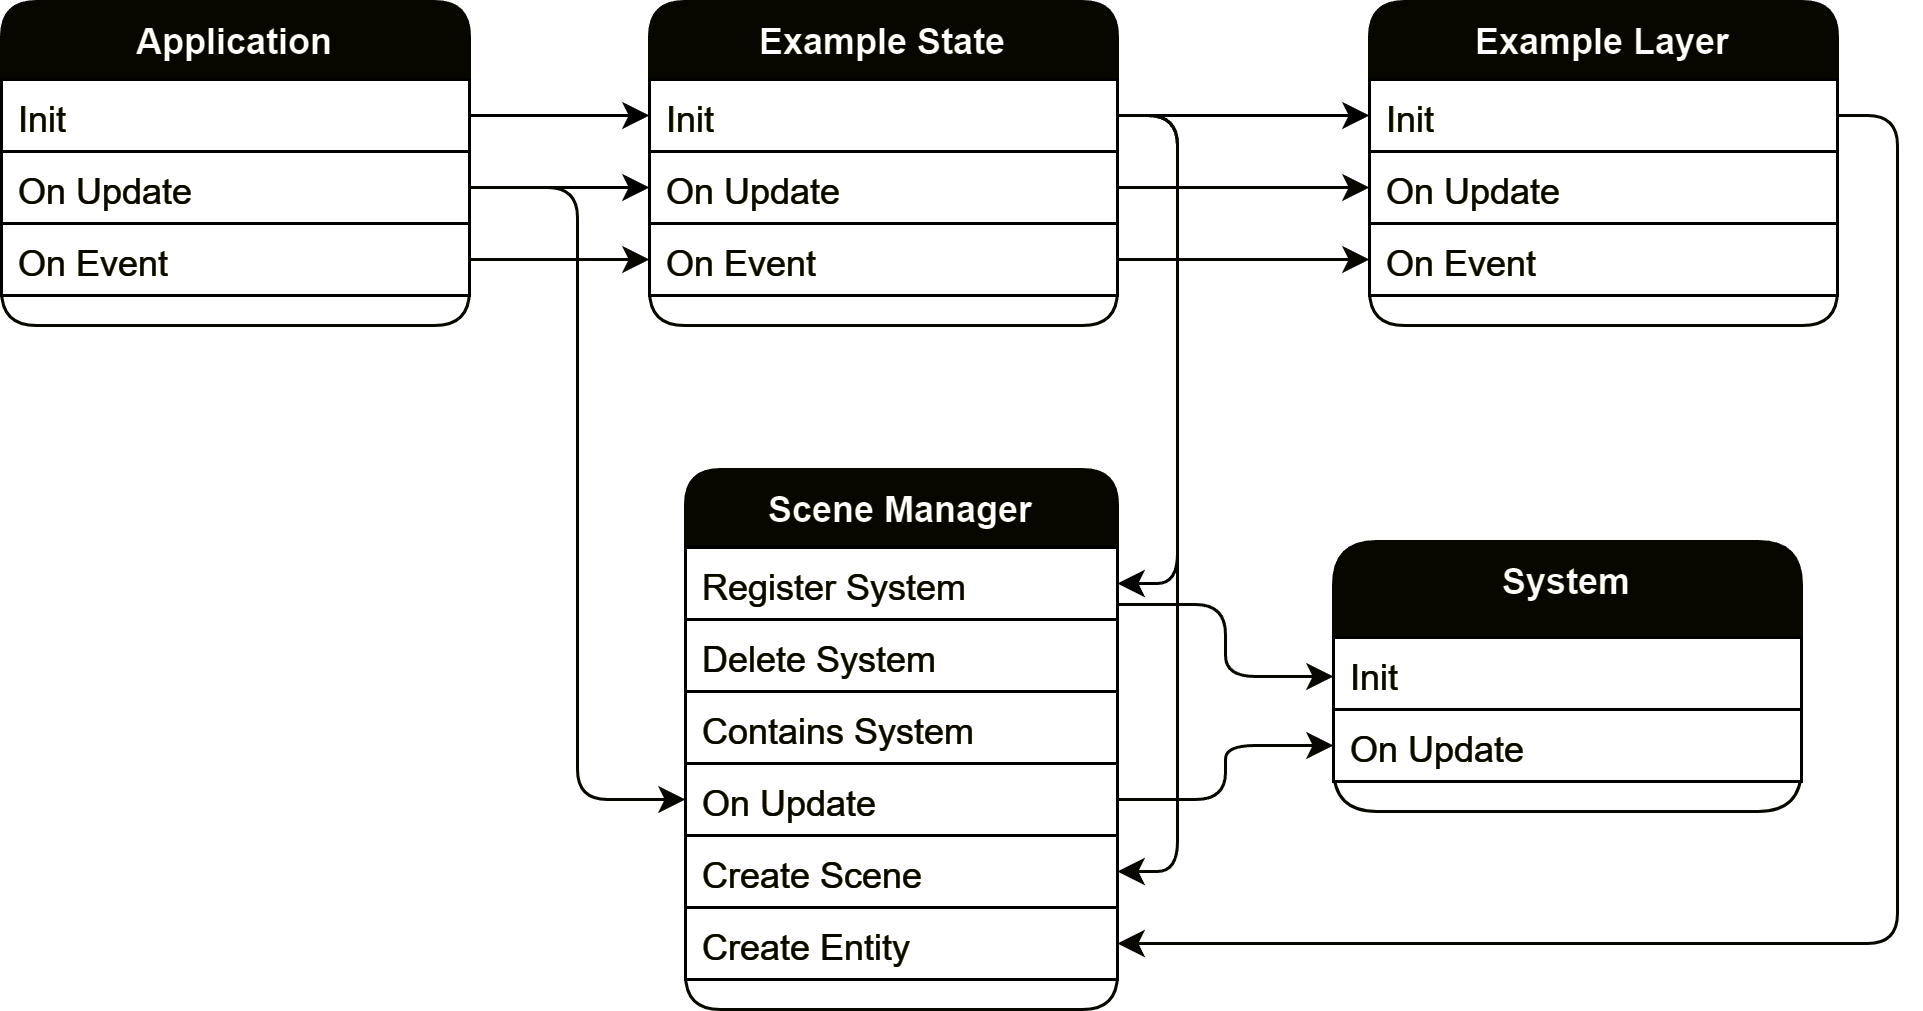
\includegraphics[scale=0.17]{engine_workflow}
    \caption{Flujo actualización y eventos}
    \label{engine_workflow}
\end{figure}

\section*{4.4. Flujo Debugger}\addcontentsline{toc}{section}{4.4. Flujo Debugger}\label{sec:workflow_debugger}

El \textit{debugger} ofrece al usuario la posibilidad de analizar en detalle lo que ocurre en el motor y la lógica de su juego
en tiempo de ejecución, usando para ellos las herramientas predefinidas o propias.

\subsection*{4.4.1. Inspector}\addcontentsline{toc}{section}{4.4.1. Inspector}\label{sec:workflow_debugger_inspector}

El inspector permite al usuario navegar entre diferentes paneles para analizar el estado del motor.

El panel \textit{assets manager} \figurename~\ref{assets_inspector} 
permite ver cada \textit{asset} cargado en memoria, para un \textit{asset} escena se podrá ver los
\textit{assets} y entidades definidas en el archivo JSON, o para un \textit{asset} textura se podrá
visualizar la imagen y sus propiedades.

\begin{figure}[h!]
    \centering
    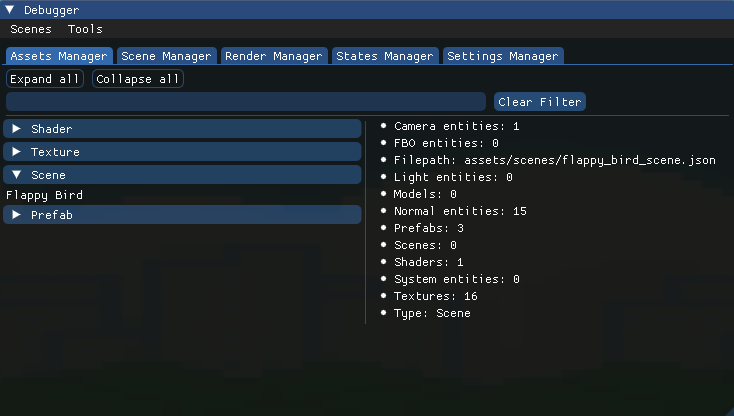
\includegraphics[scale=0.65]{assets}
    \caption{Inspector de assets}
    \label{assets_inspector}
\end{figure}

El panel \textit{scene manager} \figurename~\ref{scene_inspector} 
permite ver los elementos que componen la escena: Prefabs, Sistemas, Prototipos e Instancias.

\begin{figure}[h!]
    \centering
    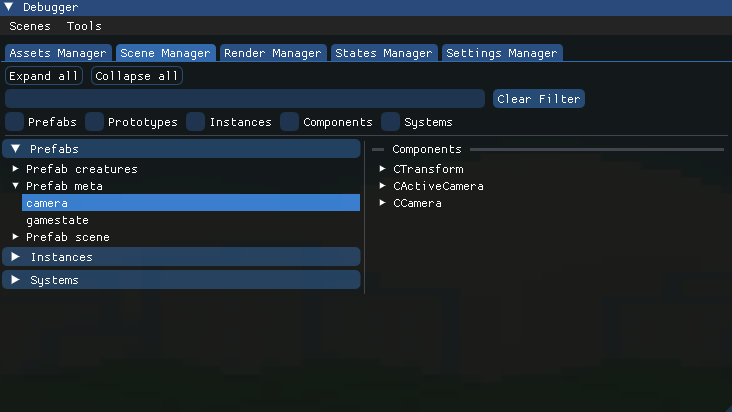
\includegraphics[scale=0.65]{escena}
    \caption{Inspector de escena}
    \label{scene_inspector}
\end{figure}

El panel \textit{render manager} \figurename~\ref{render_inspector} 
muestra información sobre elementos relacionados con el motor gráfico.

\begin{figure}[h!]
    \centering
    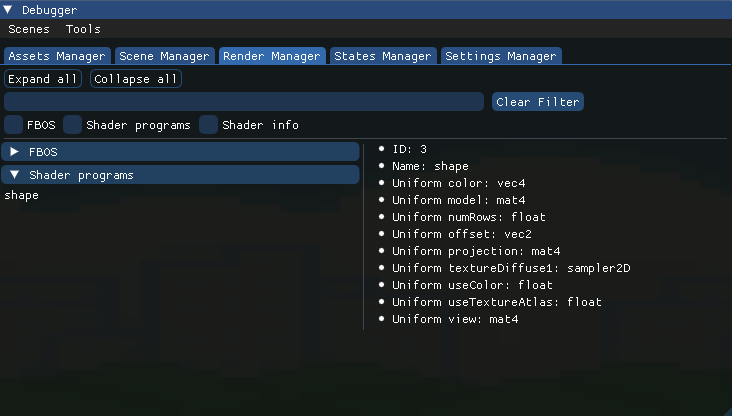
\includegraphics[scale=0.65]{render}
    \caption{Inspector del motor gráfico}
    \label{render_inspector}
\end{figure}

El panel \textit{states manager} muestra el estado actual y los \textit{layers} activos, por ejemplo en la \figurename~\ref{states_inspector}
se puede ver el estado \textit{Menú} y los \textit{layers} con los botones y las imágenes del estado.

\begin{figure}[h!]
    \centering
    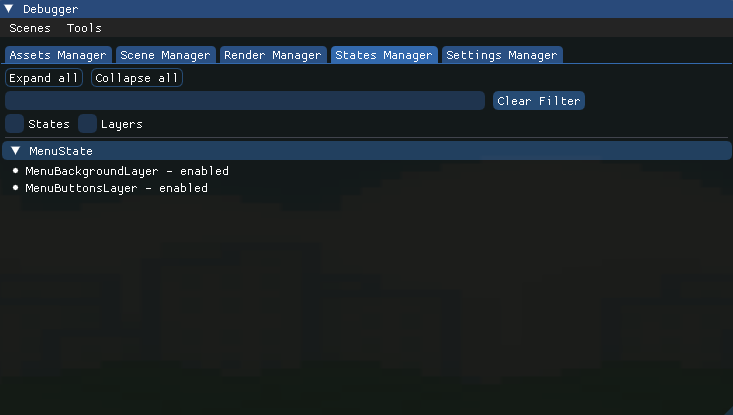
\includegraphics[scale=0.65]{estados}
    \caption{Inspector de la máquina de estados}
    \label{states_inspector}
\end{figure}

\newpage
\vfill

El panel \textit{settings manager} permite configurar las opciones del motor y la aplicación \figurename~\ref{settings_inspector}.

\begin{figure}[h!]
    \centering
    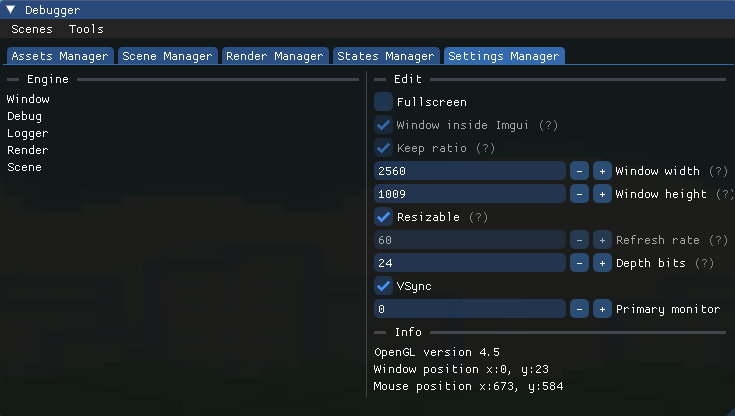
\includegraphics[scale=0.65]{settings}
    \caption{Inspector de configuración}
    \label{settings_inspector}
\end{figure}

\subsection*{4.4.2. Métricas}\addcontentsline{toc}{section}{4.4.2. Métricas}\label{sec:workflow_debugger_metrics}

La herramienta métricas \figurename~\ref{metrics_tool} muestra el rendimiento de la aplicación, 
la escena, los \textit{assets} cargados en memoria por tipo, el motor gráfico y el hardware del ordenador ejecutando el motor.

\begin{figure}[h!]
    \centering
    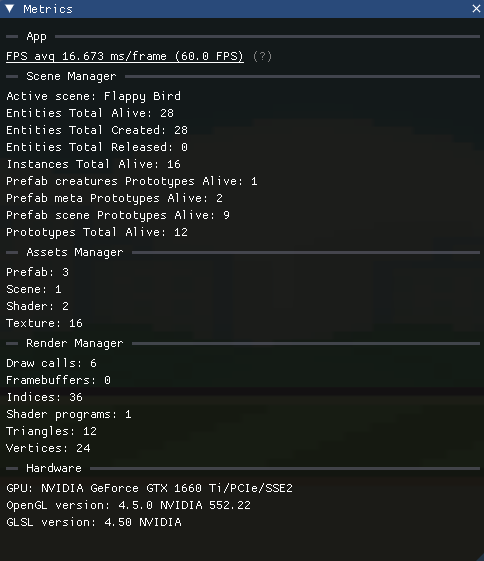
\includegraphics[scale=0.60]{metricas}
    \caption{Herramienta Métricas}
    \label{metrics_tool}
\end{figure}

\subsection*{4.4.3. Logger}\addcontentsline{toc}{section}{4.4.3. Logger}\label{sec:workflow_debugger_logger}

La herramienta \textit{logger} \figurename~\ref{logger_tool} permite leer los logs generados por el motor y la aplicación
con las siguientes opciones:
\begin{itemize}
    \item Filtrar por nivel de log, tiempo y texto.
    \item Configurar la información que se muestra sobre los logs por columnas.
    \item Opciones para copiar y borrar logs.
\end{itemize}

\begin{figure}[h!]
    \centering
    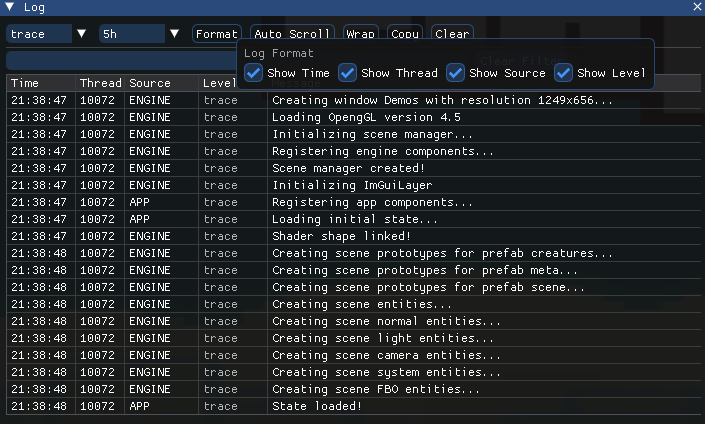
\includegraphics[scale=0.60]{logger}
    \caption{Herramienta Logger}
    \label{logger_tool}
\end{figure}

\emptyPage